\chapter{Założenia wstępne}
\label{ch:zalozenia-wstepne}

W rozdziale tym przedstawiono opis wymagań funkcjonalnych i niefunkcjonalnych, które określają, jakie zadania system musi spełniać oraz jakie kryteria jakościowe są wymagane do zapewnienia prawidłowego działania platformy mobilnej. Omówiono również schemat funkcjonalny aplikacji, opis wykorzystanego sprzętu elektronicznego oraz metodykę pracy i etapy projektu.


\section{Wymagania funkcjonalne i niefunkcjonalne}
Wymagania funkcjonalne odnoszą się do kluczowych funkcji systemu, które muszą zostać spełnione, aby system mógł realizować swoje podstawowe zadania. W przypadku autonomicznej platformy mobilnej do sortowania klocków funkcje te obejmują między innymi:
\begin{itemize}
    \item Rozpoznawanie kolorów klocków – system musi identyfikować kolory klocków przy pomocy kamery i odpowiednich algorytmów przetwarzania obrazu (czerwony, zielony, niebieski).
    \item Przekierowywanie klocków – po rozpoznaniu koloru, system kieruje klocek do odpowiedniego pojemnika.
    \item Samodzielne poruszanie się – robot powinien nawigować w wyznaczonej przestrzeni zgodnie z zaprogramowanymi trasami.
\end{itemize}

Wymagania niefunkcjonalne obejmują kryteria jakościowe, które determinują, jak system ma działać. Są to:

\begin{itemize}
    \item Niezawodność – system powinien pracować nieprzerwanie przez określony czas bez błędów.
    \item Szybkość przetwarzania obrazu – analiza obrazu i detekcja koloru muszą odbywać się na bieżąco, co jest szczególnie istotne w przypadku szybkich linii produkcyjnych.
\end{itemize}

\section{Przypadki użycia i diagramy UML}

Poniższy diagram zawiera schamam funkcjonalny aplikacji. Wyszczególniono na nim najważniejsze funkcjonalności oraz prawdopodobne możliwe zdarzenia. Szczegółowa obsługa błędów nie została wprowadzona ze względu na chęć utrzymania dobrego poziomu czytelności schematu. 

\begin{figure}[h]
    \centering
    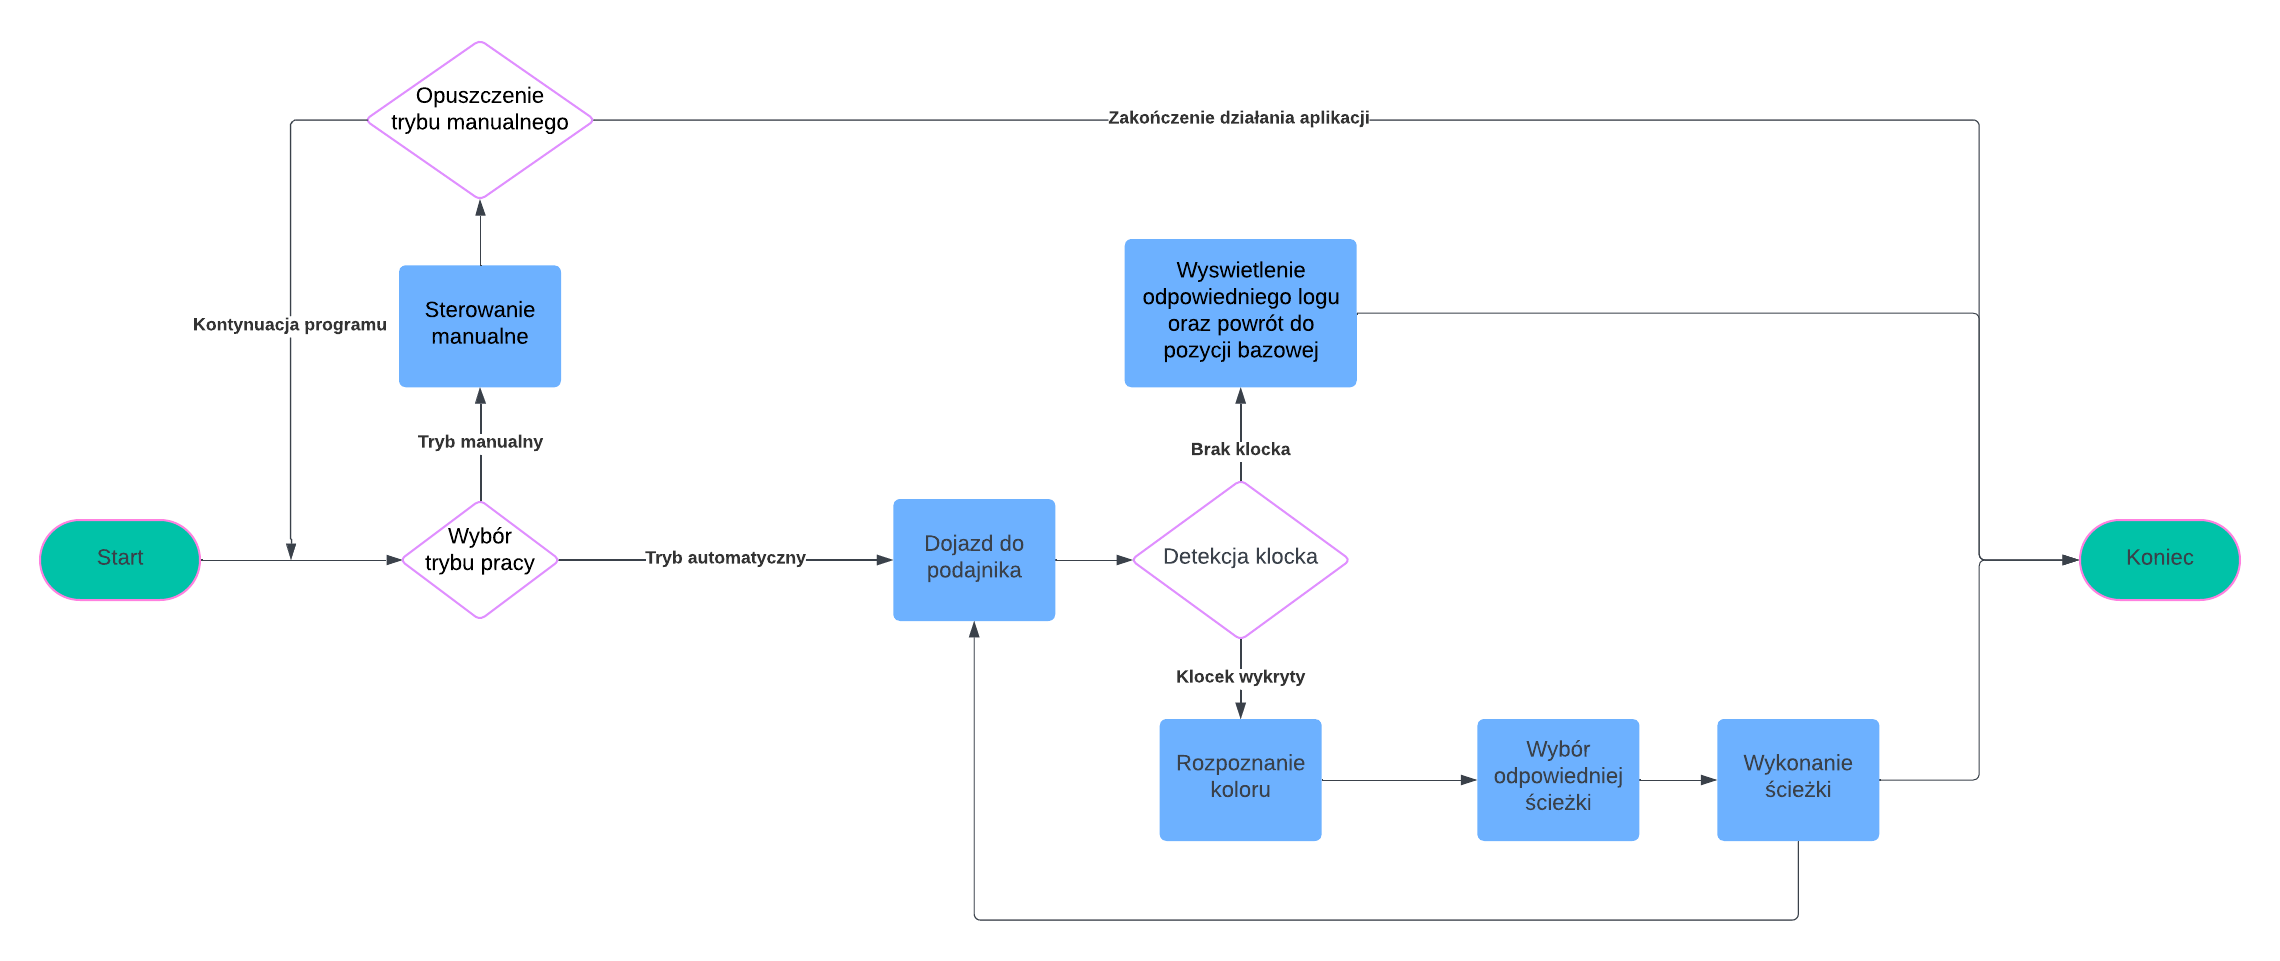
\includegraphics[width=1.0\textwidth]{./graf/uml.png}
    \caption{Schamat UML zawierający podstawowe funkcjonalności}
    \label{rys1:schemat_uml}
\end{figure}

\section{Opis wykorzystanego sprzętu elektronicznego}
W projekcie wykorzystano wiele urządzeń elektronicznych w celu zapewnienia wymaganej funkcjonalności. Szczegółowa lista wraz z opisem każdego z urządzeń znajduje się poniżej:

\begin{itemize}
    \item Raspberry Pi – służy jako główny komputer zarządzający systemem, wyposażony w odpowiednie moduły do obsługi kamery oraz komunikacji.
    \item Arduino UNO R3 - mikrokontroler pełniący rolę kontrolera napędów oraz enkoderów.
    \item Cytron MDD10A - sterownik silników odpowiadający za generowanie odpowiednich sygnałów PWM oraz dostarczenie wymaganego napięcia do silników DC.
    \item Kamera Sony IMX519 16 Mpx - element odpowiadający za akwizycję obrazu oraz umożliwienie wykorzystania wizji komputerowej. 
    \item Silniki DC Pololu 20,4:1 12V HP 25Dx65L - elementy wykonawcze robota mobilnego wyposażone w enkodery magnetyczne kwadraturowe działające na podstawie efektu Hall'a.
    \item Serwomechanizm DS3218 MG - element wykonawczy, którego zadaniem jest zamykanie oraz otwieranie chwytaka.
    \item Przetwornica Step-Up/Step-Down 5V S13V30F5 - element konieczny do poprawnego zasilenia układu SBC z pakietu ogniw litowo-jonowych.
    \item Ogniwa litowo-jonowe typu 16850 - Pakiet składający się z czterech ogniw połączonych szeregowo odpowiada za zasilanie robota podczas pracy. 
    \item Płytka stykowa - element umożliwiający wygodne wyprowadzenie pasma zasilającego enkodery oraz serwomechanizm. 
    \item Przewody połączeniowe. 
    
\end{itemize}

\section{Metodyka pracy i etapy projektu}
Projekt został zrealizowany zgodnie z metodyką iteracyjno-przyrostową, co umożliwiło sukcesywne rozwijanie i weryfikację funkcjonalności na poszczególnych etapach w rzeczywistych warunkach roboczych systemu. Na każdym etapie projektowania, implementacji oraz testowania gromadzono informacje zwrotne na temat działania systemu. Zebrane dane pozwalały na identyfikację obszarów wymagających poprawy, co skutkowało dostosowaniem parametrów systemu lub optymalizacją kodu w celu zapewnienia optymalnej wydajności.

Prace rozpoczęto od przygotowania środowiska programistycznego oraz poprawnego połączenia kamery z mikrokontrolerem Raspberry Pi. Na tym etapie skupiono się na konfiguracji narzędzi do programowania i przetestowaniu prawidłowego działania kamery. Był to kluczowy element, gdyż precyzyjny odczyt obrazu miał wpływ na późniejsze funkcje rozpoznawania kształtów i kolorów.

Kolejnym krokiem było podłączenie elementów wykonawczych oraz implementacja aplikacji kontrolującej silniki i enkodery, które stanowiły podstawę sterowania ruchem robota. Po wdrożeniu sterowników przeprowadzono wstępne testy napędu różnicowego, analizując dokładność przemieszczenia oraz reagowanie systemu na sygnały z enkoderów. 

Następnie wykonano prototyp podwozia robota, aby sprawdzić działanie algorytmów sterowania w kontekście rzeczywistych warunków pracy. Użycie prototypu pozwoliło ocenić efektywność sterowania, jak i stabilność ruchu, co przyczyniło się do dokonania wczesnych poprawek w konstrukcji oraz kodzie. Po przeprowadzeniu testów prototypowych zaprojektowano właściwe podwozie i wydrukowano je w technologii druku 3D, umożliwiając integrację z wcześniej skonfigurowanymi komponentami elektronicznymi i mechanicznymi.

W kolejnych iteracjach skupiono się na dalszym testowaniu i optymalizacji programu kontrolera silników, co pozwoliło uzyskać wymaganą precyzję i stabilność pracy napędu. 

Po uzyskaniu satysfakcjonujących rezultatów w zakresie sterowania przystąpiono do projektowania górnej części obudowy robota, która miała za zadanie stabilne zamocowanie kamery oraz częściowe osłonięcie komponentów wewnętrznych. 

Ostatecznym etapem była pełna integracja wszystkich komponentów systemu oraz finalne testy funkcjonalne. Testy obejmowały analizę wszystkich kluczowych funkcji robota w warunkach rzeczywistych, umożliwiając ocenę pracy systemu jako całości oraz identyfikację ostatnich potencjalnych usprawnień. Cały proces zakończył się uzyskaniem gotowego rozwiązania, które spełniało założenia projektowe i osiągało zamierzoną funkcjonalność.
